\documentclass[12pt]{article}

\usepackage{pablo-devoir}
\usepackage[a5paper,margin=2cm]{geometry}

\pagestyle{empty}

\title{Fonctions affines Vecteurs}
\date{04/02/15}
\classe{2\up{des}14}
\dsnum{DM 4}

\begin{document}

\maketitle

\begin{exercice}[Équation de fonction]~
  \begin{enumerate}
    \item Calculer l'équation de la droite $\cal D$ passant par les points $A(\frac{1}{3}; 2)$ et $B(1; \frac{2}{3})$.
    \item Dresser le tableau de signe de la fonction.
    \item Dans un repère orthonormé, placer les points $A$, $B$, et tracer la droite $\cal D$. Vérifier la cohérence des réponses données aux questions précédentes.
  \end{enumerate}
\end{exercice}

\begin{exercice}[Tableau de signe]~

  Tracer la courbe d'une fonction (pas nécessairement affine) qui puisse correspondre au tableau de signes suivant.

      \begin{center}
        \begin{tikzpicture}
          \tkzTabInit[lgt=2,espcl=2]
          {$x$ /1,
            $f(x)$ /1
          }
          {$-2$,$3$, $5$, $10$, $12$}%
          \tkzTabLine{, -, z ,+ ,z,-,z,+}
        \end{tikzpicture}
      \end{center}
\end{exercice}

\begin{exercice}[Vecteurs]
  Soient $ABCD$ un quadrilatère quelconque, et $I$, $J$, $K$, $L$ les milieux respectifs de $[AB]$, $\left[ BC \right]$, $\left[ CD \right]$ et $\left[ DA \right]$.

  \begin{enumerate}
    \item Faire une figure.
    \item À l'aide (entre autres) de la relation de Chasles, montrer que $\vecteur{IJ}=\frac{1}{2}\vecteur{AC}$.
    \item De même, montrer que $\vecteur{LK}=\frac{1}{2}\vecteur{AC}$.
    \item En déduire la nature du quadrilatère $IJKL$.
    \item Quelle propriété du collège venez-vous de démontrer ?
  \end{enumerate}
  

\end{exercice}

\end{document}
